\cotefile{156-5}
\scanpage{2}
\mspage{1}
\margin{GF V}
% slanted
\margin{\uline{Algèbre} des \uline{figures}}
\uline{Sorite ensembliste}. \quad (14.6.86)

Soient $L$ un, $\unsure{\mathscr{L}|\mathcal{L}}\subset\unsure{\mathcal{P}|\mathscr{P}}(L)$ ens de parties de $L$. Posons
\[
|\mathscr{L}|=\deleted{\unsure{\mathscr{L}}}\bigcup_{A\in\mathscr{L}}A
\]
et pour $A\in\mathscr{L}$
\[
\partial A=\bigcup_{\substack{B\in\mathscr{L}\\B\subset A}}B,\qquad A^\circ=A\setminus\partial A
\]

% slanted
\margin{Voir variante ``indexée'' \uline{formellement} \uline{plus forte}, voir GF \uline{VIII}, \unsure{pg|p} 37....}
\uline{Proposition 1} Les conditions suivantes sont équivalentes :

$1^\circ)$ Pour tout $x\in L$, \deleted{dans l'ens $\mathscr{L}_x$ des} \inserted{l'ensemble}
\[
\mathscr{L}_x=\{A\in\mathscr{L}\mid x\in A\}
\]
admet un plus petit élément, (noté $A(x)$).

$2^\circ)$ \deleted{\unsure{Pour}}On a les deux conditions

\[
\alpha)\ \forall A,B\in\mathscr{L},\quad\text{on a}\quad
 A\cap B=\bigcup_{\substack{C\in\mathscr{L}\\C\subset A\cap B}}C
\]
$\beta)$ $\forall x\in\mathscr{L}$, il existe un élément \uline{minimal} de $\mathscr{L}_x$ i.e. un $A\in\mathscr{L}$ tel que $x\in A^\circ$ -- i.e.
\[
\bigcup_{A\in\mathscr{L}}A^\circ=\unsure{(\mathscr{L})|\lvert\mathscr{L}\rvert}.
\]

$3^\circ)$ On a les \deleted{deux}\inserted{trois} conditions suivantes

(où \deleted{\unsure{\ensuremath{\mathscr{L}'}}} on a posé
\[
\mathscr{L}'=\{A\in\mathscr{L}\mid A^\circ\ne\varnothing\}
\]
$\gamma)$ La famille $\{A^\circ\}_{A\in\mathscr{L}'}$ forme une \uline{partition} de $|\mathscr{L}|$, i.e. $\forall x\in\unsure{\lvert\mathscr{L})|\lvert\mathscr{L}\rvert}$, \deleted{\unsure{\ensuremath{\exists!}}} existe un \uline{unique} $A\in\mathscr{L}'$ tel que $x\in A^\circ$, i.e.
\[
\bigcup_{A\in\mathscr{L}'} A^\circ=|\mathscr{L}|\quad\text{et}\quad
(A,B\in\mathscr{L}^{\unsure{*|\prime}},\ A^\circ\cap B^\circ\ne\varnothing)\Rightarrow(A=B)
\]

\margin{NB On peut remplacer $\delta,\eta$ par $(\delta')$ $\forall A\in\mathscr{L}$, on a $A=\displaystyle\bigcup_{\substack{B\in\mathscr{L}\\B\subset A}}B^\circ$}
\[
\left\{\begin{aligned}
\delta)&\quad \deleted{\text{Tout}}\,\forall A\in\mathscr{L},\quad A\ \text{est saturé dans }|\mathscr{L}|\\
 &\quad\text{pour la relation d'équivalence précédente.}\\
\eta)&\quad\text{Si } A,B\in\mathscr{L},\quad A^\circ\subset B\ \text{et }\
 \underset{\text{i.e. } A\in\mathscr{L}'}{\underbrace{A^\circ\ne\varnothing}}\ \Rightarrow A\subset B
\end{aligned}\right.
\]
\scanpage{3}
\mspage{2}
\uline{Dém}

$1^\circ\Rightarrow 2^\circ$ \quad Supposons $1^\circ$, \deleted{\unsure{on}}Prouvons $\alpha)$ et $\beta)$

$\alpha)$ Soit $x\in A\cap B$, donc $A(x)\subset A$, $A(x)\subset B$, donc
\[
 x\in C\subset A\cap B\qquad\text{d'où}\qquad A\cap B=
 \bigcup_{\substack{C\in\unsure{\mathscr{L}|\mathcal{L}}\\C\subset A,B}}C
\]

$\beta)$ trivial

$2^\circ)\unsure{\Rightarrow|=}3^\circ)$ \quad Prouvons $\gamma)\,\text{et})\ \delta),\eta)$

$\gamma)$ On sait $\displaystyle\bigcup_{A\in\mathscr{L}'}A^\circ=\bigcup_{A\in\mathscr{L}}A^\circ=|\mathscr{L}|$ par $\beta)$, prouvons que $A,B\in\mathscr{L},\ A^\circ\cap B^\circ\ne\varnothing\Rightarrow A=B$. Soit $x\in A^\circ\cap B^\circ$. Prouvons $A=B$ il suffit de prouver que $x\in A^\circ$ \deleted{$\Rightarrow A$ plus \unsure{pet|pet.}} i.e. $A$ minimal dans $\mathscr{L}_x$, implique que $A$ est un plus petit élément de $\mathscr{L}_x$. Soit $B\in\deleted{\unsure{B_x}}\mathscr{L}_x$, donc $x\in\deleted{\unsure{A^\circ}}B\deleted{\unsure{{}_x}}$ \deleted{\unsure{et}} $\Rightarrow$ $x\in A^\circ\cap B\subset\unsure{A'|A}\cap B\underset{\alpha}{=}\displaystyle\bigcup_{\substack{C\in\mathscr{L}\\C\subset A,B}} C$,
Comme $x\in C$, par le car. minimal de $A$ on a $C=A$, comme $C\subset B$ on a $A\subset B$, OK.

$\delta)$ Soit $A\in\mathscr{L}$, $x\in A$, \deleted{prouvons que $A(x)^\circ\subset A$} \deleted{i.e. $B\subset$} \inserted{considérons} l'unique $B\in\mathscr{L}'$ tel que $x\in B^\circ$, il faut prouver que $B^\circ\subset A$, or on vient de voir que \deleted{$B$ est \unsure{i|:}} $x\in B^\circ\Rightarrow B$ est plus petit élément dans $\mathscr{L}_x$ ; donc on a $\deleted{B=}B\subset A$, donc $B^\circ\subset A$, qed.

\inserted{$\eta)$ A été vu en cours de route : si $x\in A^\circ$, $x\in B$, alors $A\subset B$.}

$3^\circ\Rightarrow1^\circ$. \quad On suppose $\gamma)$ et $\delta)$ prouvons $1^\circ)$. Soit $x\in|\mathscr{L}|$, par $\gamma)$ $x$ appartient à un unique $A^\circ$ \unsure{*|x|,} $(A\in\mathscr{L}')$, prouvons que $A$ est plus petit él de $\mathscr{L}_x$. Soit $B\in\mathscr{L}$ tel que $x\in B$, il faut prouver $A\subset B$. \deleted{Comme} Par $\delta$ $B$ est saturé donc $x\in B$, $x\in A^\circ\Rightarrow A^\circ\subset B$. \deleted{Il faut donc prouver que $A^\circ$} Par $\eta$, on a $A\subset B$,
\scanpage{4}
\mspage{3}
\uline{\unsure{Remarque|Remarques}} \deleted{Si \unsure{de|dans} \unsure{\textcircled{1}} $2^\circ)$,} \inserted{$1^\circ)$} La condition $\beta)$ de $2^\circ$ est automatique si $\unsure{\mathscr{L}|\mathcal{L}}$ fini, plus gén. si $\mathscr{L}$ est ``artinien'' pour $\subset$, i.e. s'il n'existe pas de suite str. décroissante d'éléments de $\mathscr{L}$
\[
 A_1\supset A_2\supset\ldots
\]
Si par contre $\mathscr{L}$ est réduit à \deleted{\unsure{une telle}} \inserted{\unsure{l'ens des}} termes d'une telle suite, \deleted{\unsure{alors} \illegible{1}} alors $\alpha$ est satisfaite mais non $\beta$ si $\displaystyle\bigcap A_i\ne\varnothing$.

$2^\circ)$ Dans $3^\circ$, \deleted{il suffit de supposer} la condition $\eta)$ n'est pas surabondante,
\[
\left\{\begin{aligned}
 &\deleted{\displaystyle\bigcup_{A\in\mathscr{L}'}A^\circ=|\mathscr{L}|}\\
 &\deleted{\displaystyle\forall A\in\mathscr{L},\ \text{on a } A=\bigcup_{\substack{B\in\mathscr{L}\\\text{t.q. }B^\circ\subset A}}B^\circ}
\end{aligned}\right.
\]
comme on voit dans l'exemple suivant
\[
\deleted{\mathscr{L}=\{A,B,C,D\}\quad\text{\deleted{\unsure{de}} \unsure{sur|où}}\ L=\{x,y,z,t\}}
\]
\figure{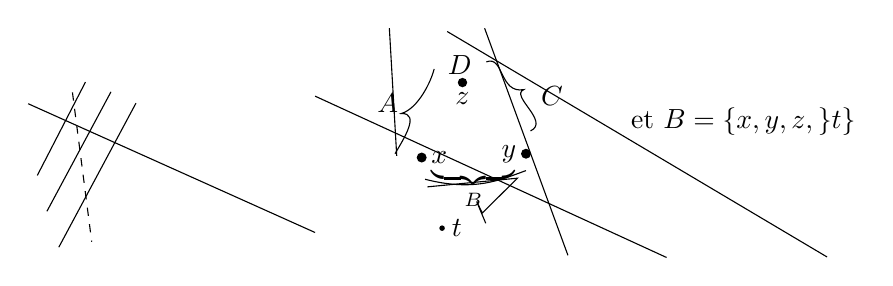
\begin{tikzpicture}[x=0.72cm,y=0.69cm,baseline]
\node at (2.05,2.18) {$\deleted{D}$};
\fill (2.10,1.85) circle (1.7pt) node[below] {$\deleted{z}$};
\fill (1.38,0.47) circle (1.8pt) node[right] {$\deleted{x}$};
\fill (3.22,0.54) circle (1.8pt) node[left] {$\deleted{y}$};
\fill (1.74,-0.83) circle (1pt) node[right] {$\deleted{t}$};
\node at (0.78,1.47) {$\deleted{A}$}; \node at (3.68,1.60) {$\deleted{C}$};
\draw (1.60,2.10) .. controls (1.55,1.88) and (1.32,1.37) .. (1.02,1.28)
 .. controls (1.36,1.29) and (1.06,.81) .. (.91,.54);
\draw (2.52,2.23) .. controls (2.83,2.36) and (2.75,1.64) .. (3.18,1.72)
 .. controls (2.93,1.61) and (3.65,1.13) .. (3.30,.96);
\node at (2.29,-.10) {$\deleted{\unsure{\underbrace{\hspace{3em}}_{B}}}$};
\draw (1.44,.07) .. controls (2.30,-.16) and (2.75,.05) .. (3.22,.23);
\draw (1.48,-.07)--(3.07,.09)--(2.45,-.55)--(2.35,-.34)--(2.51,-.74);
\node[right] at (4.9,1.14) {\deleted{et $B=\{x,y,z,\deleted{\unsure{\}}}t\}$}};
\draw[thin] (-4.55,1.86)--(-5.40,.14) (-4.10,1.68)--(-5.23,-.52) (-3.66,1.47)--(-5.02,-1.18);
\draw[dashed,thin] (-4.78,1.67)--(-4.44,-1.08);
\draw[thin] (-5.56,1.46)--(-.5,-.91);
\draw[thin] (-.5,1.60)--(5.70,-1.37); \draw[thin] (1.83,2.79)--(8.53,-1.36);
\draw[thin] (.81,2.85)--(.94,.50); \draw[thin] (2.49,2.85)--(3.96,-1.33);
\end{tikzpicture}}
\[
\deleted{A^\circ=\{x\},\ C^\circ=\{y\},\ D^\circ=\{z\},\ B^\circ=
\deleted{\unsure{\varnothing|\{z\}}}\{t\}}
\]
% slanted
\margin{Exemple idiot -- mais voir contre\unsure{xemple|exemple} correct (avec I \uline{infini}) GF \uline{VIII}, p\unsure{ges|ages} 44,45.}
\[
\begin{aligned}
 &\deleted{\mathscr{L}=\{A,B,C,D\}\qquad\text{avec}}\\
 &\deleted{A\cap C=D,\quad\deleted{\unsure{D|A}\unsure{\subset|=}\,B}}
\end{aligned}
\]
\diagram{\begin{tikzcd}[ampersand replacement=\&,row sep=1.1em,column sep=1em]
 \& \deleted{D} \arrow[dl,no head,bend right=45,shorten <=2pt,shorten >=2pt] \arrow[dr,no head,bend right=48,shorten <=2pt,shorten >=2pt] \& \\
 \deleted{A} \& \& \deleted{C} \arrow[dl,no head,bend left=8] \\
 \& \deleted{\unsure{B}}\deleted{B} \&
\end{tikzcd}}
\deleted{donc}
\[
\begin{aligned}
 &\deleted{\deleted{A^\circ=A\setminus D,\ \unsure{t|1}}}\\
 &\deleted{D^\circ=D,\ A^\circ=A\setminus D,\ C^\circ=C\setminus D,\ B^\circ=B\setminus(A\cup C)}
\end{aligned}
\]
\deleted{\deleted{On a $A^\circ\subset B$} On a $A^\circ\subset B$ mais non pas $A\subset B$. Ici \deleted{$A^\circ$} tous les $X^\circ$ $(X\in\mathscr{L})$ sont non vides.}

\margin{\deleted{[\unsure{\ensuremath{\delta}|\ensuremath{\eta}} \unsure{et} si $A\in\mathscr{L}\Rightarrow A\ne\varnothing$ ??]}}
\uline{Définition} On dit que $\mathscr{L}$ est \uline{préadmissible}, si elle satisfait les conditions équivalentes $1^\circ,2^\circ,3^\circ$. \unsure{!} On dit qu'elle est \uline{admissible} si de plus
\scanpage{5}
\mspage{4}
\unsure{pour} \deleted{\unsure{le}}\unsure{tt|\ensuremath{\forall}} $A\in\unsure{\mathscr{L}|\mathcal{L}}$, on a $A^\circ\ne\varnothing$. (Donc l'ens d'indices de la partition de $3^\circ)\,\gamma$ est $\mathscr{L}$ lui-\ensuremath{=})

\deleted{\uline{Proposition 2} Soient $\mathscr{L},\Psi$ deux familles préadmissibles. Conditions équivalentes :}

% slanted
\margin{Souvent il est plus commode de dire que c'est un \uline{préordre} sur $S$ -- $I$ est \unsure{l'ens.} ordonné associé, $\unsure{R|\mathscr{R}}_{\mathscr{L}}$ la \unsure{rel.} \unsure{d'éq.} \unsure{d'équivalence|dite} \unsure{associée}, \unsure{pour|par} le \unsure{préordre|préordonné}. Les $A\in\mathscr{L}$ sont les parties fermées \uline{irréd.}}
% slanted
\margin{\uline{NB} Se donner une famille \uline{pré}admissible, c'est se donner un système comme dessus (\deleted{\unsure{qui corres}} \inserted{où} $I=\mathscr{L}'=\{A\in\mathscr{L}\mid A^\circ\ne\varnothing\}$) et de plus, un ens. \unsure{fini|fin.} \deleted{de \unsure{parti}} $\Psi$ de parties fermées de $I$ (\unsure{correspondant} aux éléments de $\mathscr{L}\setminus\mathscr{L}'$)}

Se donner dans $L$ une famille admissible \inserted{$\mathscr{L}$} de parties, revient au $=$ que de se donner

a) Un ens ordonné $I$ \qquad (une copie conforme de $\mathscr{L}$)

b) Une partie $S$ de $L$ \qquad ($S=|\mathscr{L}|$)

c) Une application surjective $\unsure{\varphi|\phi}:S\unsure{\text{---}|\longrightarrow}I$ \quad ($x\mapsto A(x)$)

Prenant sur $I$ la top. associée à l'ordre (où les fermés sont les réunions quel\uline{conques} d'ens. $I_{\leq i}$, les ouverts les réunions quelc. d'ens $I_{\geq i}$) -- donc $\uline{\ensuremath{J\subset I}}$ est fermé ssi $\deleted{\unsure{\forall}}i\in J,\ j\leq i\Rightarrow j\in J$) et sur $S$ la top. image inverse (qui est aussi celle définie par le préordre induit de l'ordre de $I$ via $\varphi$), \deleted{les} on récupère $\deleted{\unsure{P}}\mathscr{L}$ comme
\[
 \mathscr{L}=\left\{\overline{\varphi^{-1}(i)}=\varphi^{-1}
 \bigl(\overline{\{i\}}=I_{\leq i}\bigr)\right\}_{i\in I}
\]
(indexation fidèle). Les parties fermées de $S$ sont les réunions quelconques \deleted{de} ``strates fermées'' i.e d'éléments de $A$, elles correspondent \deleted{\unsure{d|1} à \unsure{un|un*}}\inserted{biuniv.} aux parties fermées \inserted{$J$} de $I$ ($\unsure{\simeq|\cong}$ \deleted{de} $\mathscr{L}$), \inserted{par transp. inv. par $\varphi$} \deleted{les parties ouvertes sont les correspondants aux}
\[
\deleted{\unsure{X}}A_J=\bigcup_{i\unsure{\leq|\in}J}A_i
 =\underset{\substack{\text{si on identifie}\\I=\mathscr{L},\ \text{donc }J\subset\mathscr{L}}}{\bigcup_{A\in J} A}
 =\underbrace{\deleted{\unsure{\bigcup}}\bigsqcup_{i\in J}A_i^\circ}_{\substack{\text{réunion}\\\text{disjointe}\\\text{de parties}\\\text{non vides}}}
\]
\uuline{NB} \deleted{Si on regarde les}

De $=$, les parties ouvertes sont celles de
\scanpage{6}
\mspage{5}
la forme
\[
 \deleted{\unsure{X}}A_J=\bigcup_{i\in J}A_i^\circ={\unsure{\varphi|\phi}}^{-1}(J)
 \tag*{(1)}
\]
où $\deleted{\unsure{A}}J$ est une partie ouverte de $I$ (ou de $\unsure{\Phi|\Psi|\mathscr{L}}\simeq I$) (\deleted{\unsure{bien}} sûr, cette fois dans $\displaystyle\bigcup_{i\in J}$ il n'est pas question de remplacer $A_i^\circ$ par $A_i$ !). Les parties loc. fermées sont de \ensuremath{=} les
\[
 \deleted{\unsure{X}}A_J=\varphi^{-1}(J)=\bigcup_{i\in J}A_i^\circ
\]
où cette fois $J$ est une partie loc fermée de $I$, i.e. telles que
\[
 i\leq j\leq k,\quad i,k\in J\quad\Rightarrow\quad j\in J
 \tag*{$(*)$}
\]
(les $\deleted{\unsure{J|I}}I_{\geq i}$, $i\in J$, sont des ouvert de $I$ recouvrant $J$, et \deleted{\unsure{dans cet}}\inserted{pour un tel} ouvert, \deleted{$J$}\inserted{$J\cap I_{\geq i}$} est fermé \inserted{dans $I_{\geq i}$,} à cause de $(*)$, donc $J$ est bien loc. fermé si on a $(*)$, l'inv. étant encore plus évident \ldots)

\uline{NB} On peut aussi dire, \inserted{si $\unsure{\mathscr{L}|\mathcal{L}}$ fini,} que les $A^\circ$ $(A\in\mathscr{L})$ sont les \deleted{\unsure{at}} fibres de l'algèbre de Boole engendrée par les $A\in\mathscr{L}$ dans $\unsure{\mathcal{P}|\mathscr{P}}(S)$ $(S=|\mathscr{L}|)$. Les ens obtenus à partir des $A\in\mathscr{L}$, par réunions, intersections et \unsure{complémentaires|complémentations} dans $S=\unsure{\lvert\mathscr{L})|\lvert\mathscr{L}\rvert}$, sont exactement ceux saturés par la rel d'équiv. dans $S$ définie par les $\unsure{A^\circ|X^\circ}$ \unsure{i.e.|id.} celle définie par $\varphi$. Donc ils correspondent biuniv. aux parties quelc. de $I$, par la forme
\[
 J\longmapsto A_J=\varphi^{-1}(J)=\bigcup_{i\in\unsure{J|\supset}}A_i^\circ .
\]
On \unsure{appelera|appellera} \unsure{ses|ces|les} ens \unsure{ainsi|aussi} les \uline{parties} $\mathscr{L}$-\uline{modérées} ou $\mathscr{L}$-\uline{constructibles} de $\mathscr{L}$.
\scanpage{7}
\mspage{6}
\unsure{``} \uline{Sous-famille} \inserted{(ou sous-ens)} \uline{admissible} d'un ens admissible $\unsure{\mathscr{L}|\mathcal{L}}\subset\unsure{\mathcal{P}|\mathscr{P}}(L)$ : par définition, c'est un $\Psi\subset\mathscr{L}$ qui est \uline{fermé} dans $\mathscr{L}$. Alors pour $A\in\Psi$, $\deleted{\unsure{\partial_{\mathscr{L}}A}}$ on a
\[
 \partial_{\Psi}A=\partial_{\mathscr{L}}A\quad\text{donc}\quad
 A^{\circ(\deleted{\mathscr{L}}\Psi)}=A^{\circ(\mathscr{L})},
\]
ce qui montre que $|\Psi|$ est une partie saturée de $|\mathscr{L}|$, pour la rel. d'équiv. $\deleted{\unsure{\mathscr{L}}}R_{\mathscr{L}}$ \unsure{\ensuremath{s=}|sur|\ensuremath{S=}} $|\mathscr{L}|$,
\deleted{La top. de $\Psi$ est induite}

En fait, avec les notations précédentes, on a
\[
 |\Psi|=A_\Psi
\]
\deleted{De \ensuremath{=}, il est évident que pour \unsure{ce|x}} Soit $x\in|\Psi|$, donc $\deleted{\unsure{A}}\exists A\in\Psi$ tel que $\unsure{a|x}\in A$, \deleted{$x\in|\Psi|\Rightarrow$} et donc $x\in A(x)\subset A$ (puisque $A(x)$ est le plus petit des éléments de $\mathscr{L}$ qui $\ni x$) donc $A(x)\in\Psi$ ($\Psi$ étant fermé). Donc $A(x)$ est aussi le plus petit élément \uline{de $\Psi$} qui contient $x$ :

\deleted{\unsure{Ain}} Ainsi, $\Psi$ est préadmissible, et de plus il est évident que il est admissible (les $A^{\circ\Psi}\ne\varnothing$, d'après $A^{\circ(\Psi)}=A^{\circ\mathscr{L}}$).

\uline{Prop.} Soit $\mathscr{L}\subset\mathcal{P}(L)$ ens de parties admissible, et soit $\Psi\subset\mathcal{P}(L)$. Conditions équivalentes

a) $\Psi\subset\mathscr{L}$, et $\Psi$ est une partie fermée de $\mathscr{L}$

b) $\Psi\subset\mathscr{L}$, $\Psi$ est admissible, \inserted{$|\Psi|$ est saturé dans $|\mathscr{L}|$ pour $\unsure{R_{\Psi}|R_{\varphi}|R_{\mathscr{L}}}$,} et la relation d'équivalence \inserted{$R_\Psi$} \unsure{sur|de} $|\Psi|\subset|\mathscr{L}|$ définie par $\Psi$ est celle induite par $R_{\mathscr{L}}$
\scanpage{8}
\mspage{7}
On vient de voir que $a)\Rightarrow b)$ prouvons l'inverse, supposons $b)$ prouvons $a)$ i.e. soient $A\in\Psi$, $B\in\unsure{\mathscr{L}|\mathcal{L}}$, $B\deleted{\unsure{\in}}\subset A$ prouvons $B\in\Psi$

Considérons $B^\circ$, on a $B^\circ\ne\varnothing$ ($\Psi$ adm.) et comme $R_\Psi=R_{\mathscr{L}}\lvert\deleted{\unsure{\mathcal{P}|B}}\Psi\rvert$ \inserted{\unsure{saturé|saturée}}, on a $B^\circ=C^\circ$ pour $C\in\deleted{\mathscr{L}}\Psi$ convenable, puis cela implique $\deleted{\unsure{C}}B=C$, donc $B\in\Psi$, qed.

On dit que $\Psi$ est une \uline{sous-famille} \uline{admissible}.

\uline{Scholie} Elles correspondent \inserted{(avec conservation des rel. d'ordre)} aux parties fermées de $\mathscr{L}$, ou de $|\mathscr{L}|$. \unsure{\ensuremath{\Rightarrow}|=}\,Elles sont \uline{stables} par $\cup$ et $\cap$ quelc. dans $|\mathscr{L}|$.

\uline{Proposition} Soient $\mathscr{L},\Psi\subset\unsure{\mathcal{P}|\mathscr{P}}(L)$ deux ens de parties admissibles. Conditions équiv.

a) $\mathscr{L}\cup\Psi$ est admissible, et $\mathscr{L},\Psi$ en sont deux sous-ens. admissibles (i.e. fermés)

\inserted{$\deleted{\unsure{a}}a')$ $\mathscr{L}$ et $\Psi$ sont \deleted{\unsure{deux}}\unsure{sous}-familles adm. d'une famille \inserted{adm.} $\Sigma$}
b) $\mathscr{L}\cap\Psi$ est $\mathscr{L}$-fermé dans $\unsure{\Phi|\mathscr{L}}$ et \inserted{$\Psi$-fermé} dans $\Psi$,
\[
 \text{et}\qquad |\mathscr{L}|\cap|\Psi|=|\mathscr{L}\cap\Psi|
\]
c) $|\mathscr{L}|\cap|\Psi|$ est $\mathscr{L}$-fermé dans $|\mathscr{L}|$ et \ensuremath{\{} $\Psi$-fermé dans $\Psi$, et \deleted{\unsure{toute} $A\in\mathscr{L}$ telle} \deleted{pour} pour $A\subset|\mathscr{L}|\cap|\Psi|$, $A\in\mathscr{L}$ \deleted{de $\mathscr{L}$} ssi $\unsure{A|1}\in\Psi$, (i.e. ssi $A\in\mathscr{L}\cap\Psi$).

% slanted
\margin{Cf condition équiv. \unsure{pg|pge} 11 (genre d), ``strate par strate''}
\deleted{d) $\forall A\in\mathscr{L}, B\in\Psi$, on ait $\unsure{A}\ \mathscr{L}_{\unsure{\leq A|<A}}$ et $\Psi_{\unsure{\leq|<}}$}

$a')\Leftrightarrow a)$ évident par les sorites précédents de \ensuremath{=} que $a)$ implique $b)$ et $c)$. Reste à prouver $b\Rightarrow c$, $c\Rightarrow a$.

Prouvons d'abord $b\Rightarrow c$. Comme $|\mathscr{L}|\cap|\Psi|=\lvert\mathscr{L}\cap\Psi)$ par $b)$, et $\mathscr{L}\cap\Psi$ fermé dans $\mathscr{L}$ et
\scanpage{9}
\mspage{8}
fermé dans $\Psi$, il s'ensuit que $\lvert\unsure{\mathscr{L}|\mathcal{L}}\cap\Psi\rvert$ est fermé dans $\lvert\mathscr{L}\rvert$ et fermé dans $\lvert\Psi\rvert$.. Soit $A\in\mathscr{L}$, $A\subset\lvert\mathscr{L}\rvert\cap\lvert\Psi\rvert=\lvert\unsure{\Phi|\mathscr{L}}\cap\Psi\rvert$, on a donc par le sorite préliminaire (comme $\mathscr{L}\cap\Psi$ fermé dans $\Psi$) que $A\subset\displaystyle\bigcup_{\deleted{\unsure{C}}B\in\mathscr{L}\cap\Psi}B$, cela implique \deleted{que $A\ \exists!$} (comme les $B$ dans $\mathscr{L}$) que $\exists\,B\in\mathscr{L}\cap\Psi$ tel que $A\subset B$.
\deleted{Appliquant le \ensuremath{=} raisonnement à $B$ (qui est $\unsure{\in|\subset}\mathscr{L}\cap\Psi$ donc $\subset\lvert\Phi\cap\Psi\rvert=\lvert\mathscr{L}\rvert\cap\lvert\Psi\rvert$) on} Mais comme $\mathscr{L}\cap\Psi$ est \deleted{\unsure{f}}$\Psi$ fermé dans $\Psi$, on en conclut $A\in\Psi$, qed.

$c\Longrightarrow a$ \quad On suppose c), prouvons a).

$1^\circ)$ $\mathscr{L}\cup\Psi$ est admissible. Soit $x\in\lvert\mathscr{L}\cup\Psi\rvert=\lvert\mathscr{L}\rvert\cup\lvert\Psi\rvert$ \deleted{\inserted{Si $x$} soit $A(x)$ le plus} Si $x\in\lvert\mathscr{L}\rvert\cap\lvert\Psi\rvert$, soit $A(x)$ le plus petit élément de $\mathscr{L}$ tel que $x\in A(x)$, et \unsure{itout|itou}. $B(x)\in\Psi$ \unsure{..,|.,} $x\in B(x)$. Comme $T=\lvert\mathscr{L}\rvert\cap\lvert\Psi\rvert$ est $\mathscr{L}$-fermé dans $\lvert\mathscr{L}\rvert$, on a $A\deleted{\unsure{\in}}(x)\subset T$, et de $=$ $B(x)\subset T$. On doit donc avoir (par c) $A(x)\in\Psi$ ie \deleted{$A(x)\in\mathscr{L}\cap\Psi$, et} donc par définition de $B(x)$ on a $\deleted{\unsure{A}}B(x)\subset A(x)$, de $=$ $A(x)\subset B(x)$, \inserted{soit $\unsure{C|D}$}
\deleted{donc} \inserted{\unsure{donc}} Cela montre que $C$ est le plus petit élément de $\mathscr{L}\cup\Psi$ qui conti\deleted{\unsure{ennent|enne}}\inserted{ent} $x$. Il reste à prouver que si $A\in\mathscr{L}\cup\Psi$, alors \deleted{$A$ n'est \unsure{p|pas}} \[
 \bigcup_{\substack{B\in\mathscr{L}\cup\Psi\\B\subsetneq A}}B
 \ne\deleted{\unsure{C|B}}A^{\text{\deleted{\unsure{ce|car}}}} .
\] \deleted{Mais} Il \deleted{$A\in\mathscr{L}$, $\unsure{\Psi|B}$ \illegible{3} $B\subset A$} suffit pour ceci de prouver que \inserted{si \unsure{(p. ex.)|(p.ex)} $A\in\mathscr{L}$,} les $B$ en
\scanpage{10}\mspage{9}
en question sont dans $\unsure{\mathscr{L}|\Phi}$, i.e. que $\mathscr{L}$ est fermé dans $\mathscr{L}\cup\Psi$ (et itou pour le cas $A\in\Psi$, avec $\Psi$ fermé dans $\mathscr{L}\cup\Psi$). Donc il vient

\[
\begin{aligned}
2^{\circ})\quad &\deleted{\unsure{\Psi}}\mathscr{L}\ \text{fermé dans }\mathscr{L}\cup\Psi:\quad A\in\mathscr{L},\ B\in\Psi,\\
&B\subset\deleted{\unsure{B}}A\ \Longrightarrow\ B\in\deleted{B}\mathscr{L}.
\end{aligned}
\]
Mais on aura $\deleted{\unsure{\lvert B\rvert}}$ $B\subset\lvert\mathscr{L}\rvert\cap\lvert\Psi\rvert$, donc $B\in\mathscr{L}\Rightarrow B\deleted{\unsure{\subset}}\in\deleted{\unsure{\mathscr{L}}}\Psi$ OK.

\uline{\unsure{Définition|Definition}} On dit alors que $\mathscr{L}$ et $\Psi$ \uline{compatibles}

\uline{Corollaire \unsure{1|!}} Quand ces conditions sont satisfaites, $\lvert\deleted{A}\mathscr{L}\rvert\cap\lvert\Psi\rvert$ est une partie de $\lvert\mathscr{L}\rvert$ qui est $\mathscr{L}$-saturée, et une partie de $\Psi$ qui est $\Psi$-saturée, et les deux relations d'\unsure{équivalence|équilence} induites par $\lvert\deleted{\unsure{B}}\mathscr{L}\rvert$ et par $\lvert\Psi\rvert$ sont les $=\mathrm{s}$.

Mais attention, cette dernière condition ne suffit nullement à impliquer que $\mathscr{L}$ et $\Psi$ compatibles. Exemple : $\mathscr{L}$ et la famille \inserted{$\mathscr{L}^{\circ}$} des $A^{\circ}$ ont $=$ support, et définissent la $=$ relation d'équiv. sur $\lvert\mathscr{L}\rvert$, mais elles ne sont compatibles que si elles sont \uline{égales} \deleted{(car} i.e. $\mathscr{L}$ formé d'ens. deux à deux disjoints. En effet \deleted{(car la relation d'ordre sur $\mathscr{L}$ et sur $\mathscr{L}^{\circ}$ n'est la $=$ que si}

\uline{Corollaire 2} Supposons $\mathscr{L}$ et $\Psi$ compatibles. Alors $\lvert\mathscr{L}\rvert\subset\lvert\Psi\rvert$ sss $\mathscr{L}\subset\Psi$, $\lvert\mathscr{L}\rvert=\lvert\Psi\rvert$ sss $\mathscr{L}=\Psi$.
\scanpage{11}\mspage{10}
En \deleted{\unsure{l}}effet, c'est connu pour les sous-familles admissibles d'une famille (ici $\unsure{\mathscr{L}|\Phi}\cup\deleted{\unsure{\mathscr{L}}}\Psi$) -- cf. Scholie \unsure{pge|pg} 7.

\margin{\uline{Cor} 3 Si $\mathscr{L},\Psi$ comp., alors pour $\mathscr{L}',\deleted{\unsure{\Psi}}\leq\mathscr{L},\ \Psi'\leq\Psi$ (parties fermées) $\mathscr{L}'$ et $\Psi'$, st admissibles, et $\mathscr{L}'\cup\Psi'$ est fermé (ss-famille adm.) dans $\mathscr{L}\cup\Psi$.}

% slanted
\margin{On appellera ainsi les éléments de $\unsure{\mathcal F|\mathscr F}$ les \uline{``figures ensemblistes''} de $L$}

Soit $\mathcal F$ l'ens des \deleted{toutes} les parties \uline{admissibles} $\mathscr{L}$ de $\unsure{\mathcal P|\mathfrak P}(L)$. On ordonne $\mathcal F$ par
\[
\begin{aligned}
\mathscr{L}\leq\Psi\quad\overset{\mathrm{def}}{\Longleftrightarrow}\quad &\mathscr{L}\ \text{est une ss-}\\
&\text{famille admissible}\\
&\text{de }\Psi.
\end{aligned}
\]

Alors on a

\uline{C 1} $\mathcal F$ admet des Sup majorés, car si $\mathscr{L}_i\in\mathcal F,\ \mathscr{L}_i\leq\deleted{\mathscr{L}}\Psi$ des ss-ens. fermés d'un $=$ $\deleted{\mathscr{L}}\Psi$, alors $\bigcup_i\mathscr{L}_i$ est un sous-ens. fermé de $\Psi$, qui est le la sup. C'est immédiat par \unsure{le sorite|les sorites} sur les sous-familles \unsure{équiv.|égaux.} (\unsure{de ses|i.e.|les|deux} parties fermées) d'un $\Psi$

% slanted
\margin{La Sup pour la relation $\leq$ (qui est ici $\subset$) est $\bigcup_i$}

\deleted{\unsure{Oui|Or|O.K.}, un peu \unsure{vif|cf.}, il faut \unsure{passer|préciser} par des Sup finis, en notant que $\emptyset\subset\mathcal P(L)$ est admissible (! cas du Sup \inserted{de la fam.} vide !) -- la seule famille admissible $\underset{\in\mathcal F}{\mathscr{L}}$ telle que $\lvert\mathscr{L}\rvert=\emptyset$ et que si $\mathscr{L},\Psi,\Sigma$ sont tels que}

% slanted
\margin{\unsure{explicitons|expliciter} \unsure{cf.} \uuline{Prop} ou Cor}

% This line has a horizontal cancellation in addition to the diagonal strokes across the draft.
\deleted{$\mathscr{L}$ et $\Psi$) est admissible, alors $\Sigma$ \unsure{ai|est}}

\deleted{($\mathscr{L},\Psi$) compatibles, alors $\Sigma$ est compatible avec $\mathscr{L}\unsure{\cup|et}\Psi$ \unsure{sss|ssi} il l'est avec $\mathscr{L}$ et avec $\Psi$}
\scanpage{12}\mspage{11}
Les éléments irréductibles de $\unsure{\mathcal F|\mathscr F}$ sont les $\unsure{\mathscr{L}|\Phi}\in\mathcal F$ qui ont \deleted{\unsure{une}} un plus grand élément : car un ens fermé est irréductible (au sens fort) sss il a un plus grand élément.

% slanted
\margin{Appelons-les les ``multistrates ensemblistes''}

Donc

\uline{C 2} Tout $\mathscr{L}\in\deleted{\unsure{\mathscr{L}}}\mathcal F$ est la sup des objets irréductibles de $\mathcal F$, à savoir des $\mathscr{L}_{X}=\{Y\in\mathscr{L}\mid Y\unsure{\subseteq|\leq}X\}$, pour $Y\in\mathscr{L}$

\uline{C 3} Soient $\deleted{\mathscr{L}}F,\deleted{\Psi}G\in\mathcal F$. Pour que $F$ et $G$ soient compatibles (i.e $F,G$ majoré) il f. et s. que $\deleted{X\in F,\unsure{\Rightarrow|\to}}$ $\forall\,\deleted{\mathscr{L}}\unsure{X|{\mathscr{L}}'}\leq F$ et $\deleted{\Psi}Y\leq G$, $\deleted{\mathscr{L}}X$ et $\deleted{\Psi}Y$ \deleted{\unsure{élé|él.}} multistrates, on ait $\deleted{\mathscr{L}}\deleted{\mathscr{L}}X$ et $\deleted{\Psi}Y$ compatibles.

En d'autres termes, que pour $X\in F,\ Y\in G$, $F_X$ et $G_Y$ soient compatibles :

\uline{Remords à prop. \unsure{pge|pg} \deleted{\unsure{9}}7} : Cond. équiv à a) b) c)

d) \deleted{\unsure{compos|comp.}} $\forall\,A\in\mathscr{L},\ B\in\Psi$, $A\cap B$ est fermé dans $A$ (pour $\mathscr{L}$ i.e pour $\mathscr{L}_A$) et en $B$ (pour $\Psi$ i.e. pour $\Psi_B$), et si $\deleted{\unsure{A}\ C\in\mathscr{L}\cup\Psi}$ $C$ est une partie de $A\cap B$, alors $C\in\mathscr{L}$ ($\Leftrightarrow C\in\mathscr{L}_A$) sss $C\in\Psi$ ($\Leftrightarrow C\in\Psi_B$) i.e $\mathscr{L}_{A\cap B}=\Psi_{A\cap B}$
\scanpage{13}\mspage{12}
\deleted{ce qui}

Composantes connexes de $M=$ ens des multistrates. Les éléments minimaux de $M$ sont ceux qui sont réduits à un seul ensemble $A$, \deleted{(qui peut être} $A\ne\emptyset$ (NB $\unsure{\mathscr{L}|\Phi}=\{\emptyset\}$ n'est pas une famille admissible !\deleted{)} Si $\mathscr{L}$ est admissible, $\emptyset\notin\deleted{\unsure{F}}\mathscr{L}$, \deleted{)} puisque $A\in\mathscr{L}\Rightarrow A^{\circ}\ne\emptyset$ a fortiori $A\ne\emptyset$)
\[
\mathscr{L}\deleted{\unsure{F_{A}|\mathscr{L}_{A}}}=\{A\}
\]

\deleted{(NB)} \deleted{(NB $F\in\unsure{F|M}\Rightarrow F\ne\emptyset$ !)}

Si $X\deleted{\unsure{\mathscr{L}|F}}\in M$, \deleted{et $A\in\deleted{\mathscr{L}}F$, alors \unsure{pour}} \inserted{$\deleted{\unsure{F}}X\subset\unsure{\mathcal P|\mathfrak P}(L)$}, et si $\deleted{F}X$ admet un \deleted{plus petit} élément minimal $A$ (p.ex. $\deleted{F}X$ fini, \inserted{on suppose $X\ne\emptyset$}) alors,
\[
\deleted{F}X_A=\{A\}\leq F
\]
\deleted{d'autre part,} donc $\deleted{F_A}$ \deleted{et} $\deleted{F}X$ et $\{A\}$ dans la $=$ comp. connexe. D'autre part, \deleted{\unsure{$\{A\}$ est}} si $A\ne L$, et si $x\in L\setminus A$, $\{A\}$ et $\{\{x\}\}$ sont dans la $=$ composante connexe, car ils sont majorés par le multistrate
\[
\bigl\{\{A\},\{\{x\}\},A\cup\{\{x\}\}\bigr\}
\]
\deleted{donc} Et pour la $=$ raison, \deleted{si} \deleted{Card} \unsure{on} voit que \inserted{$\{\{x\}\}$ pour tous les} \deleted{\unsure{tous les}} pts de $L$ sont dans la $=$ comp connexe de $L$. En résumé les $X\in M$ qui ont un plus petit élément \inserted{$A$} sont dans une $=$ composante connexe, du moment que $A\ne L$ i.e. du moment que $\unsure{X\prime|X}$ ne se réduise à $\{A\}=\{L\}$. Mais celui-ci aussi, si \deleted{Card} $L\deleted{\geq}\ne\deleted{\unsure{2|0}}\emptyset$, est dans la
\scanpage{14}\mspage{13}
$=$ comp. connexe que les $\{\{x\}\}$, comme on voit à l'aide de le multistrate
\[
\bigl\{\{\{x\}\},\{L\setminus\{x\}\}\bigr\}
\]

Si $L$ \deleted{de card. $1$,} $=\emptyset$, \deleted{$\unsure{\mathcal P|\mathfrak P}(L)$ est de} \deleted{cardi} alors $M=\emptyset$, et $M$ est connexe.

Si $\operatorname{Card}L=1$, $\mathcal P(L)=\{\emptyset,L\}$, et les $\unsure{\mathscr{L}|\Phi}\subset\mathcal P(L)$ \deleted{qui sont \unsure{des} sont que} \inserted{telles} \deleted{\unsure{$\{\mathscr{L}\}$} qui ne contiennent pas $\emptyset$} pour $\emptyset\notin\mathscr{L}$ sont $\emptyset$ et $\{L\}$. Donc $M=\{\{L\}\}$ a un seul élément, et est connexe.

Donc

\uline{Prop} Si $\operatorname{card}L\leq1$, $M$ est connexe (il est vide si $\deleted{\unsure{\mathrm{Card}}}L=\emptyset$, il est de card $1$ donc $0$-connexe si $\operatorname{card}L=1$). Si $\operatorname{card}L\geq1$, alors les $\deleted{\unsure{Y|F}}X\in M$ qui ont un élément minimal sont tous dans la $=$ comp. connexe. Donc si on se borne aux \deleted{familles} figures ensemblistes \uline{finies} (ce qui n'offre pas d'inconvénient à mes yeux) $M$ est connexe. Donc l'axiome C4 \deleted{est ici de} relatif à la décomposition de $M$ en comp. connexes (que $X,Y$ appartenant à des composantes différentes sont compatible) est automatique.
\scanpage{15}\mspage{14}
Si on ne se borne aux familles finies, \unsure{Con.|on a|ben.} encore connexité. En effet, si $X\in M$ est $\ne\{L\}$, soit $A\in X$ \unsure{tels|tel|telle} que $A\ne L$, Alors $X$ et $X_A$ dans $=$ comp \inserted{connexe et}
\[
\lvert X_A\rvert=A
\]
donc si $\deleted{\{x\}}x\in L\setminus A$, on trouve une multistrate en \unsure{prenant|posant}
\[
Z=\bigl\{B\unsure{,|;}B\cup\{x\},\{x\}\mid B\in X_A\bigr\}
\]
\margin{\unsure{.}}

\uline{NB} Construction qu'on a refait ici plusieurs fois : Soient $\deleted{X}F\in\deleted{M}\unsure{\mathcal F|\mathscr F}$, $\deleted{Y}G\in\deleted{\unsure{\mathcal G|M}}\unsure{\mathcal F|\mathcal G}$, $\lvert\deleted{\unsure{X}}F\rvert\cap\lvert G\rvert=\emptyset$, posons $F\boxtimes G=\{A\cup B\mid A\in\deleted{\unsure{X}}F,\ B\in G,\ \inserted{\text{$A$ et $B$ pas tous deux $\emptyset$}}\}$, alors $(A\cup B)^{\circ}=A^{\circ}\cup B^{\circ}$, $\partial(A\cup B)=(\partial A\cup B)\cup(A\cup\partial B)$ -- si $F$ et $G$ \deleted{sont} \deleted{des} multistrates i.e. \deleted{\unsure{admet|admettent|alors}} \deleted{\unsure{pour|par|pas}} plus grand éléments \deleted{\unsure{et que si}} $A_0,B_0$ alors $A_0\cup B_0$ est pl grd élément de $F\boxtimes G$, qui est une multistrate.

\deleted{Celle-ci contient \unsure{en|un} \unsure{l}} $F\boxtimes G$ contient $F\unsure{\amalg|\sqcup}G$ comme sous-figure. Donc, si $F$ et $G$ sont des multistrates ``disjointes'' elles sont dans la $=$ comp. connexe car \unsure{disjointes|majorées|dominées} par $F\boxtimes G$. Donc en tous cas, \margin{)} $M$ connexe ($=$ sans \deleted{\unsure{la|les}} limiter aux \deleted{familles} figures ensemblistes finies).
\scanpage{16}\mspage{15}
Supports et cosupports.

$F$ et $G$ de $\unsure{\mathcal F|\mathscr F}$ sont \uline{disjoints} \inserted{(au sens de $\leq$)} sss $\lvert F\rvert\cap\lvert G\rvert=\emptyset$. Donc les $F$ disjoints d'une famille de figures $G_i$, sont celles qui \deleted{sont} satisfont $\lvert F\rvert\subset L'$, où $L'=L\setminus\bigcup_i\lvert G_i\rvert$. Donc, on voit que les supports correspondent aux parties quelconques $L'$ de $L$, la \unsure{relation|notion} de complémentarité est la notion ensembliste.

\deleted{Le $\mathcal F(L'$} L'ens des figures \inserted{de $L'$} de support $\subset L'$ \deleted{est} s'identifie aux figures de $L'$, i.e. on trouve les $\mathcal F(L')\subset\mathcal F(L)$ comme sous-ens. saturés (au sens de $\leq$ et de la disjonction \ldots).
% Paper watermark; sideways and faint; partial impressions, not manuscript prose.
\margin{\unsure{RONG}\quad\unsure{EXTRA STR}}
\scanpage{17}\mspage{16}
On récupère l'\unsure{ens} $\unsure{\mathcal P|\mathfrak P}(L)$ en termes de $L_{\leq}$, ou de $(M_{\leq},\text{compatibilité})$,

\margin{\uline{NB} $\unsure{\mathcal F|\mathscr F}$ est formé des \uline{toutes} les parties fermées de $\deleted{\unsure{\mathcal F}}M$ dont deux élémts quelc. sont comp.}

et on retrouve la relation d'ordre sur $\mathcal P(L)$ en termes de la relation d'ordre sur les supports, et itou pour \unsure{les passages|le passage} au complémentaire. Mais cela ne redonne pas directement $L$, mais $\widehat L$, le compactifié de Stone ($L$ se récupère \inserted{cependant} comme l'\unsure{ens} des points \uline{isolés} de $\widehat L$). Ceci suggère de \unsure{refaire|faire} théorie en termes d'un espace compact \deleted{\unsure{tot}} discontinu $X$, et \deleted{\unsure{de}} prendre $\mathcal F$ familles admissibles dans $X$ fermés et même à la \unsure{\uline{fois}|fois} \uline{ouverts} et \uline{fermés}.

Si on ne permet que les familles finies, alors les supports \deleted{\unsure{et}} \inserted{et les \unsure{cosupports|supports} des telles \deleted{familles} figures} s'identifient aux parties à la fois ouv. et f. de $X$. Mais
% slanted
\margin{\unsure{ou d'une|ou d'ens} \unsure{fam.|famille|finie} de telles figures}
si on permet des figures infinies ou des ens de figures infinis on les \unsure{change} en retrouvant \deleted{\unsure{à nouveau}} \inserted{les \unsure{intérieurs}} des parties \inserted{\uline{fermées}} quelconques de $\unsure{X|L}$, \unsure{ou|pour} les \deleted{paires} couples support-cosupport s'identifient aux \deleted{paires} \inserted{couples} $(U,V)$ d'ouverts de $X$,
\[
\begin{aligned}
& U=\operatorname{int}(\overbrace{\unsure{\mathrm f|\mathrm F}U}^{\inserted{\overline U}})=\operatorname{ext}V,\quad
 V=\operatorname{int}(\mathrm f\,U)=\operatorname{ext}U,\\
& \overset{\inserted{\unsure{-\ \smile\ \mathrm m|-\ \smile\ \mathrm{en}}}}{\overline U\cap\overline V} = X\setminus\{U\cup\unsure{V|X}),
\end{aligned}
\]
i.e. les \unsure{ouvert|ouverts} $U$ tels que $\overline U\unsure{\geq|= }\operatorname{int}(\overline U)$
\scanpage{18}\mspage{17}
\deleted{\unsure{14|4}} \uline{15 juin}

On peut remplacer $\unsure{\mathcal F|\mathscr F}$ par divers\deleted{\unsure{es}} \inserted{\unsure{passage|pass. ge} à une} sous-ensembles ordonnés, stables \uline{par} \deleted{$\unsure{\leq|\in}$} \deleted{et} \deleted{par Sup}
sous-figures \deleted{fermées}\inserted{(i.e. \unsure{fermés|fermé} dans $\mathcal F$)} et par $\mathrm{Sup}$.

Exemples : Si $\unsure{L|\mathcal L}$ est un esp. top. \inserted{(str. top.)}, \deleted{de}
on peut soumettre les $A\in F$ \deleted{\unsure{figur}} ($F$ figure)
à des conditions de nature topologiques, comme d'être fermés, ou \deleted{\illegible{1}} compacts, ou fermés et connexes. Toute condition
portant sur la nature des strates $A\in F$ (en tant que partie de $L$, et non en tant que multistrate\ldots), ou $=$ sur la nature des
multistrates $F_A$ $(A\in F)$, définit une sous ens. ordonné de $\mathcal F$ ayant les propriétés de stabilité voulues. Signalons ici
des propriétés \unsure{portant} sur \unsure{la|le} $A^\circ=A\setminus\partial A$ (la définition de $A^\circ$ dépend de la multistrate $F_A$), comme celle d'être \deleted{non vide} \deleted{\unsure{connexé|connexe}},
\deleted{\unsure{ou}} \deleted{\unsure{ou}} connexe, ou plus gén. $i$-connexe $\unsure{0|-1}\leq i\leq+\infty$, \deleted{\unsure{$(-1)$-connexe signifiant non vide}} \inserted{et idem pour les $A$ eux-mêmes}. Ou on peut demander aux $|\partial A|$
d'être des sphères topologiques etc.
% slanted
\margin{\uline{NB} \deleted{Mais \unsure{l'axiome|l'énoncé} de \unsure{fi.|pr.} \unsure{supposé} d'\unsure{emblée}, -- peut-être \unsure{a-t-on|stat.}, ou \unsure{même} \unsure{ceci}, \unsure{ne|de} \unsure{saurait}-il \unsure{même} \unsure{convenir|voir} \unsure{en} \unsure{spécifiant} \unsure{cette} \unsure{notion} \unsure{avec|sur} des \unsure{fig.} \unsure{ou|un} $\unsure{F}$ \unsure{seulement} \uline{\unsure{préadmissibles}}.} Aussi, la condition de \uline{densité} $A=\overline{A^\circ}$ i.e. $A\subset B\Longrightarrow A^\circ\subset\overline{B^\circ}$.}

Si $L$ est \inserted{un espace} modéré, on se borne aux $\unsure{\mathscr{L}|\Phi}\subset\unsure{\mathcal P|\mathfrak P}(L)$ pour lesquels $A\in\mathscr{L}\Longrightarrow A$ partie fermée \uline{\unsure{par ordinaire|par ordre|pour ordre}} de $L$

On peut envisager aussi des conditions de nature plus globale sur $\mathscr{L}$, au cas où
\scanpage{19}\mspage{18}
$L$ est muni d'une topologie, comme celle d'être \uline{localement} fini. Le sous-ens.
ordonné ${\unsure{\mathcal F|\mathscr F}}'$ \deleted{de} $\mathcal F$ est alors stable par sup \unsure{fini|finis}, mais pas \deleted{par} \unsure{généralt} par sup.
quelc. \uline{Figure finie} $F$ : \deleted{finie} $F$ fini au sens ordinaire, i.e. un \unsure{ens|nb} fini de strates. Figure de type fini : contenue
dans une réunion finie de ss-figures $F_A$.

\deleted{Si les strates d'une} Une figure est \deleted{\unsure{de t.}} finie \deleted{si} si et seult si elle est de t. f. et ses strates sont finies.

Autre cas : supposons $L$ muni d'une structure d'ordre -- il \unsure{--|a} dans une réalisation topologique, par des ``\uline{cellules}'' \inserted{(fermées) $X_x$ $(x\in L)$} dans un espace
top. $X$ triangulé convenable. Alors à tout $A\deleted{\unsure{\in}}\unsure{\subset|\in}L$ correspond \deleted{\unsure{le}} $X_A=\bigcup_{x\in A}X_x$.
% slanted
\margin{les $X_x$ forment une \uline{famille} admissible de parties de $X$, indexée par l'ens ordonné $L$}
On se bornera alors alors aux parties \uline{fermées} $A$ de $L$, de façon que
\[ A\longmapsto X_A \]
soit une application bijective de l'ens des parties envisagées de $L$ (les p. \uline{fermées})
\deleted{\unsure{dans l'}}\inserted{\unsure{avec un|sur un}} ens des parties \inserted{fermées} de $X$ \deleted{\unsure{stables}} \deleted{par la relation} \inserted{stables par la} relation d'équivalence \unsure{induite|induit} par \deleted{\unsure{les}} $(X_x^\circ)_{x\in L}$ (en fait, toutes les parties
\scanpage{20}\mspage{19}
de ce type si $L$ est fini). Donc on se bornera donc aux $\unsure{\mathscr{L}|\Phi}\in\unsure{\mathcal F|\mathscr F}$ telles que les $A\in\mathscr{L}$ soient fermés de $L$, i.e. telle que
\[ \mathscr{L}\subset\unsure{\mathcal P|\mathfrak P}_{\text{fermés}}(L) \]
Les \unsure{élément|éléments} de $\mathcal F'$ ainsi \unsure{obtenu|obtenus} peuvent s'interpréter en termes de $X$, comme des familles admissibles \inserted{(mais oui)} de familles de
parties \inserted{fermées} de $X$, \inserted{chacune} \uline{stables} par la relation d'équiv. des \deleted{cellules} \inserted{strates} ouvertes $X_{\unsure{\circ|a|\bullet|\cdot}}^\circ$, i.e. chacune réunion de strates fermées de $X$.
Dans une terminologie qui sera développée, elles \deleted{sont}\inserted{admettent} donc toutes le recouvrement donné de $X$ comme une ``subdivision''\unsure{;|,} (ou \unsure{plus tôt|plutôt}, \inserted{celui} induit sur leur support dans $X$)

\figure{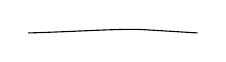
\begin{tikzpicture}\draw (0,0) .. controls (0.7,0.02) and (1.2,0.06) .. (1.5,0.04) -- (2.15,0);\end{tikzpicture}}

Soient $\deleted{\unsure{\Phi}}F$ et $G$ deux figures ensemblistes de $L$. On veut définir quand $F$ est un \uline{raffinement}, et quand c'est une \uline{subdivision} de $G$.

\uline{Proposition} Conditions équivalentes

% slanted
\margin{Cela implique $|\deleted{\unsure{A}}F|\subset|G|$}
a) $[$ $\forall\unsure{a|\cdot}\;A\in F$, désignant par $G\deleted{{}_A}{}^A$ l'ens des $B\in G$ tels que $A\subset B$, $G\deleted{{}_A}{}^A$ a un plus petit
élément $\varphi(A)$. (On trouve donc une application $\varphi:\deleted{\unsure{A}}F\longrightarrow G$, qui est bien sur croissante.) $]$ De plus
\scanpage{21}\mspage{20}
pour tout $A\in F$, $B\in G$, $A\cap F$ est \deleted{réunion de}\inserted{une} partie $F$-fermée de $|F|$, i.e. réunion de strates de $F$.
% slanted
\margin{\uline{NB} Le ``de plus'' implique déjà la première condition, si on ajoute que $|\deleted{\unsure{A}}F|\subset|\deleted{\unsure{B}}G|$, et cela équivaut à $|F|\unsure{-|\longrightarrow}|G|$ \uline{continue} (ou croissante).}\margin{Cf condition équivalente $\mathrm{b}'$) à la pge suivante}

b) Pour tout $A\in F$, $\exists\,B\in G$ telle que $A^\circ\subset B^\circ$ (strate évidemt unique, \inserted{\unsure{noté|notée|soit} $\varphi(A)$}), l'application $\varphi:\deleted{\unsure{F}}F\unsure{-|\longrightarrow}G$ ainsi obtenue est croissante (
\deleted{$A'\subset A$, et} \deleted{$A'^\circ\in\unsure{+|F}$} \deleted{$A'\subset A$} $A,\deleted{\unsure{B}}A'\in F$, $\deleted{\unsure{A'}}B,B'\in G$, \deleted{$A\unsure{\in|=|\subset} A'$, $A^\circ\subset B^\circ$, $\unsure{B\subset B'}$} avec $A^\circ\subset B^\circ$, $A'^\circ\subset B'^\circ$, $A'\subset A$, $\Longrightarrow B'\subset B$.

a) $\Longrightarrow$ b) Supposons a) prouvons b). Soit $A\in F$, \deleted{\unsure{par}} a) $\exists\ B\inserted{{}=\varphi(A)}\in G$ \deleted{tel} qui soit plus petit ds $G^A$. Prouvons $\deleted{\unsure{B}}A^\circ\subset B^\circ$. Soit
$x\in A^\circ$, il faut prouver que $B'\in G$, $B'\deleted{\unsure{\in}}\unsure{\subset|\not\subset} B$ et $x\in B'\Longrightarrow B'=B$. \deleted{Soit} Considérons $B'\cap A$, c'est une partie de $A$ réunion \unsure{de'|de} strates de $F$,
donc $\exists\ A'\in\deleted{\unsure{\Phi}}F$, telle que $x\in A'\subset B'\cap A$. Comme $x\in A^\circ$ et $A'\in\deleted{\unsure{\Phi}}F_A$, on a $A'=A$ et comme $A'=A\subset B'\cap A$, on a $A\subset B'$. D'après le caractère minimal de
$B^{\unsure{s|'}}$, on a donc $B'=B$ qed. / D'autre part, on a déjà noté que l'application $\varphi$ est croissante. \deleted{\unsure{Donc}}Cela établit b).

b) $\Longrightarrow$ a). Supposons b, prouvons a). Soit $A\in F$, soit $B\in G$ telle que $A^\circ\subset B^\circ$, prouvons que $B$ est plus petit \inserted{élémt} dans $G^A$.
% slanted
\margin{\uline{Lemme} Moyennant b) on a \unsure{(b)} : Si $A\in F$, $B\in G$, $A^\circ\subset B$ alors $A\subset B$}
Prouvons déjà que $B\in G^A$, i.e. $A\subset B$ \deleted{Soit $B'\in G$ tel que $A\subset B'$}
\deleted{Soit} On a $A=\deleted{\bigcup_{\unsure{A'}}\unsure{A^\circ}\unsure{\in|\subset}\unsure{\sim}}\bigcup_{\substack{A'\in F\\ A'\unsure{\subset|\in} A}} A'^\circ$, \deleted{Comme $A^\circ\subset B^\circ\subset B$,} il suffit de prouver que les $A'^\circ$ sont $\subset B$
\scanpage{22}\mspage{21}
Or si $B'\in G$ est tel que $A'^\circ\subset B'^\circ$, on a \deleted{$A\subset B'$} (hyp. de b) $B'\subset \deleted{A}B$, donc $A'^\circ\subset B$, OK.

Prouvons que $B$ est le plus petit él. de $G^A$. Soit $B'\in G^A$ i.e. $B'\in G$, $A\subset B'$, prouvons $B\subset B'$ ou encore $B^\circ\deleted{\unsure{\subset}}\cap B'\ne\varnothing$ \deleted{Comme}. Comme
$A^\circ\subset B^\circ$ et $A^\circ\subset A\subset B'$, on a $\underset{\substack{\mathrel{\ooalign{\hfil$\scriptstyle\shortparallel$\hfil\cr\hfil$\scriptstyle-$\hfil\cr}}\\ \varnothing}}{A^\circ}\subset B^\circ\cap B'$, OK.

Prouvons enfin que $A\in F$, $B\in G$ implique que $A\cap B$ est $F$ fermé dans $|F|$. Par b) on voit que $\underset{\substack{\shortparallel\\ \bigcup_{A\in F}A^\circ}}{|F|}\subset|G|$, et que
la relation d'équiv. $\unsure{\mathcal R|R}_F$ sur $|F|$ est plus fine que celle induite par $\mathcal R_G$ sur $|G|$. Cela implique que $A\cap B$ est saturée pour la relation d'équiv. $\deleted{\unsure{F}}\mathcal R_F$ (puisque $B$ l'est pour $\mathcal R_G$). Donc
\[ A\cap B=\bigcup_{\substack{C\in F\\ \text{t.q. } C^\circ\subset A\cap B}} C^\circ . \]
Je dis que \inserted{dans} cette réunion, \deleted{est} on peut remplacer $C^\circ$ par $C$ i.e.
\[ C\in F,\quad C^\circ\subset A\cap B\quad\Longrightarrow\quad C\subset A\cap B. \]
Comme $C^\circ\subset A$, on a $C\deleted{\unsure{{}^\circ}}\subset A$. Reste : prouver $C\subset B$. On va donner un complément \unsure{immédiat|inédit} à l'énoncé de la prop.
% slanted
\margin{Ou encore : ($\mathrm{b}''$) \unsure{On|Ou|On a} : $|F|\subset|G|$, la relation de préordre sur $|F|$ définie par $F$ est plus fine que celle induite par la relation d'ordre de $|G|$.}

\uline{Corollaire} La condition b) équivaut à
$\mathrm{b}'$) $\forall\ A\in F,\ \exists\ B\in G$ tel que $A^\circ\subset B^\circ$, et d'autre part $A\in F$, $B\in G$, $A^\circ\subset B$ implique $A\subset B$.
\scanpage{23}\mspage{22}
Il nous fallait plutôt $\mathrm b\Rightarrow\mathrm b'$ pour achever la dém. de la prop., \deleted{\unsure{Voici} \unsure{donc} \unsure{le} déjà \unsure{fait}} \inserted{et en fait on l'a déjà} \deleted{donc \unsure{à|:} voir \unsure{(pour}} \deleted{(pour $\mathrm b\Rightarrow\mathrm b'$) que}
\deleted{moyennant b), \unsure{on}}
\[ \deleted{A\in F,\quad B\in G,\quad A^\circ\subset B\quad\Longrightarrow\quad A\subset B} \]
\deleted{\unsure{On}} prouvé \deleted{\unsure{cel|cela}}en démontrant $\mathrm b)\Rightarrow\mathrm a)$ (Cf lemme marginal p. 20) Reste : prouver $\mathrm b'\Rightarrow\mathrm b$ donc moyennant $\mathrm{b}'$, le fait que $\varphi$ est croissant
\[ A,A'\in F,\quad B,B'\in G,\quad A^\circ\subset B^\circ,\quad A'^\circ\unsure{\subset|\subset'}B'^\circ,\quad \deleted{\Longrightarrow}\inserted{A'\subset A\deleted{{}^{\unsure{\circ|'|*}}}}\quad\Longrightarrow\quad B'\subset B\deleted{{}^{\unsure{\circ|'|*}}} \]
Mais \deleted{\unsure{Comme}} \inserted{par $\mathrm{b}'$) on a} \deleted{$\unsure{A^\circ\subset A^\circ|A^\circ\subset B^\circ}$ donc} \deleted{$A\subset B$, $A'\subset B'$} \deleted{$A'^\circ\subset B'^\circ$, donc par} $A\deleted{{}^{\unsure{\circ}}}\subset B\deleted{{}^{\unsure{\circ}}}$ \deleted{$\mathrm{b}'$) $A'^\circ\subset B'$, \unsure{donc} on a $A'^\circ\subset A'\subset A\subset B$ donc $A'^\circ\subset$} \deleted{$A^\circ\subset B\cap B'$, donc} donc $A'^\circ\subset B'^\circ$ \deleted{$\unsure{\subset B^\circ}\ \unsure{A\subset A'}$}
$A'^\circ\subset A\subset B$, donc $A'^\circ\subset B'^\circ\cap B$, donc $B'^\circ\cap B\ne\varnothing$, donc $B'\deleted{{}^{\unsure{\circ|'|*}}}\unsure{\in|\subset}B$, qed.

\uline{Définition} On dit, sous ces conditions, que $F$ est un \uline{raffinement} de $G$.
% slanted
\margin{\uline{NB} $F$ raffine $G$ \unsure{ssi|sss} $\forall A\in F$, $F_A$ \unsure{raff.|raffine} $G$ i.e. tt multistrate de $F$ raffine $G$.}

\uline{Ex} Toute sous figure de $G$ est un \unsure{raff.}$^{\unsure{t}}$ de $G$
Notation $F\ll G$. C'est \uline{une relation d'ordre}

\uline{Proposition} Soient $F$ et $G$ deux figures, \deleted{telles que $F$ soit un raffinement de $G$.} Conditions équivalentes
a) \inserted{$F\ll G$,} Il n'existe pas de raffinement de $G$ autre que $F$, parmi ceux dont $F$ soit une sous figure -- i.e. $F$ est \unsure{minimal|maximal} dans l'ens des raffinements de $G$, ordonné \unsure{par|pour} $\leq$ (relation de sous figure)
b) \inserted{$F\ll G$ et} $|F|=|G|$ \deleted{c) L'applicat}
\scanpage{24}\mspage{23}
b) $\Rightarrow$ a) Si $F'$ est un raffinement de $G$ tel que $F'$ sous figure de $F$, on a $|F|\subset|F'|\subset|G|$, et comme $|F|=|G|$ on
a $|F|=|F'|$, donc $F=F'$, puisque $F$ sous-figure de $F'$,
% slanted
\margin{\uline{Donnons aussi} condition équ\unsure{iv.|iv} c) \inserted{$F\ll G$ et} Toute strate de $G$ est réunion de strates de $F$. Et quand \unsure{on ne suppose plus|on ne suppose pas} \unsure{par avance|d'avance} que $F\ll G$, la condition d) \[\left\{\begin{aligned}&1^\circ)\ \text{Toute strate de }G\text{ est réunion de strates de }F\\&2^\circ)\ \forall \deleted{\unsure{B}}A\in F,\quad G^A=\{B\in G\mid B\supset A\}\text{ a un}\\&\text{plus petit élément.}\end{aligned}\right.\]}

a) $\Rightarrow$ b) Supposons que $|F|\ne|G|$, \deleted{soit $x\in|G|\setminus|F|$, considérons la} Il existe donc une figure $\deleted{F}H$ \deleted{qui soit} \inserted{telle} que \deleted{\unsure{vide}, qui soit un raffinement de $G$,}
\[ \left\{\begin{aligned} &|H|\ne\varnothing\\ &\deleted{F}H\ \text{raffine }G\\ &\deleted{F}H\ \text{disjointe de }F \end{aligned}\right. \]
par exemple on prend \unsure{un} $x\in|G|\setminus|F|$, et la figure $\deleted{F}H=\{\{x\}\}$. Or on a

\uline{Corollaire}\enspace Soient $F,H$ deux figures qui raffinent $G$, et telles que $F$ et $H$ \deleted{disjointes} \inserted{compatibles}. Alors $F\cup H$ raffine $G$.
% slanted
\margin{\figure{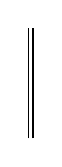
\begin{tikzpicture}\draw (0,0)--(0,1.4) (.06,0)--(.06,1.4);\end{tikzpicture}} à noter \unsure{comme|comme une|ce} propriété formelle \unsure{intéress.|intéressante}. \unsure{Cas contraire|Au contraire|Par contre} $\pm$ \unsure{génle.} \unsure{(au moins|(au voisin}, les \unsure{construction|contraires|conditions} \unsure{modérée|modérés}) des unions (cas non modéré) si $F$ et $G$ disjointes\ldots}
\inserted{\uline{Plus gén.}, ça marche pour Sup \unsure{quel.|quelc.} (au sens de $\leq$)}
En effet, on utilise le fait que les multistrates de $F\cup H$ sont les multistrates \deleted{qui sont communes à $F$} qui appartiennent à $F$, ou \deleted{à} $H$. Or la propriété de raffinement se vérifie sur les multistrates.

\uline{Définition} On dit alors que $F$ est une \inserted{\uline{subdivision}} de $G$.
\scanpage{25}\mspage{24}
Notation $F\preccurlyeq G$. C'est encore une relation d'ordre sur $\unsure{\mathcal F|\mathcal J}$.

\uline{NB} Se donner dans $L$ un couple $F\subset G$, avec $F$ raffinant $G$, revient au $=$ que de se donner
\diagram{\begin{tikzcd}[ampersand replacement=\&,column sep=large,row sep=large]
S\;(=|F|)\arrow[r,hook,"i"]\arrow[d,"p","\text{surj}"'] \& T\;(=|G|)\arrow[r,-,to path={([xshift=4pt,yshift=2pt]\tikztostart.east) .. controls ([xshift=-1pt,yshift=2pt]\tikztostart.east) and ([xshift=-1pt]\tikztostart.east) .. ([xshift=4pt]\tikztostart.east) -- (\tikztotarget.west) -- ([xshift=-2pt,yshift=2pt]\tikztotarget.west)}]\arrow[d,"q"',"\text{surj}"] \& L \\
I\;(=F)\arrow[r,"\varphi"] \& J\;(=G) \&
\end{tikzcd}}
où $S\subset T$ sont des sous. ens. de $L$, $\varphi:I\longrightarrow J$ une application \uline{croissante} d'ensembles ordonnés, et \deleted{$\unsure{p}$}
\[p:S-I,\quad q:T-J\]
des appl. \uline{surjectives} ($\varphi$ pas \unsure{néc.|nec.} surjective)

Alors l'inclusion $i$ est continue pour les top. \unsure{corresp|comp|can.} sur $S,T$ définies par leurs préordres respectifs (images inv. des top. sur $I,J$) L'image inverse d'une partie \inserted{$G$-}modérée de $T$ est une partie $F$-modérée de $S$, cette notion se \unsure{raméne|ramène} à la notion
\[J'\longrightarrow\varphi^{-1}(J')\]
au niveau des parties de $J,I$. L'image \deleted{\unsure{inv.}}dir. d'une partie fermée
